\subsection{相关社区}
\begin{itemize}
    \item \href{https://www.linuxfoundation.org/}{Linux Foundation}: Linux基金会是一个非盈利性的联盟,其目的在于协调和推动Linux系统的发展,以及宣传、保护和规范Linux
    \item \href{https://www.cncf.io/}{Cloud Native Computing Foundation}:Linux基金会旗下的非盈利组织,使命是创造和推动采用云原生计算来助力企业在云计算模式下更好的构建可扩展的应用程序。
    \item \href{https://openhpc.community}{OpenHPC}: Linux基金会旗下项目,
    关注于提供开源的HPC组件和最佳实践,以降低HPC使用门槛
\end{itemize}

\subsection{HPC相关框架}
\subsubsection{OpenHPC/ohpc}
\href{https://github.com/openhpc/ohpc}{ohpc}是OpenHPC社区维护的一套开源HPC集群部署指南,
包含操作系统置备、资源管理、开发工具、运行时等各类HPC相关组件,

\begin{itemize}
    \item 操作系统可选Rocky8、Leap15
    \item 操作系统置备可选Warewulf、xCAT\footnote{由于xCAT不支持Rocky8,当前最新\href{https://github.com/openhpc/ohpc/releases/tag/v2.5.GA}{2.5}版本不提供xCAT选项。}
    \item 资源管理可选OpenPBS、SLURM
    \item 支持x86\_64、aarch64两种架构
\end{itemize}

\subsection{Serverless框架}
目前,已经出现不少的开源serverless框架,
大多基于Kubernetes平台。
在serverless平台下,
用户只需要编写类似\cref{openfaas_helloworld}的函数来处理业务逻辑,
由平台负责进行自动调度。
\begin{figure}
\begin{minted}{python}
def handle(event, context):
    return {
        "statusCode": 200,
        "body": "Hello from OpenFaaS!"
}
\end{minted}
\caption{OpenFaaS下使用Python编写的"Hello World"}
\label{openfaas_helloworld}
\end{figure}

已知的serverless框架大致有以下几种\cite{faas_evaluation}:

\begin{table}[ht]
\begin{tabularx}{\textwidth}{|X|p{3cm}|p{2.5cm}|p{2cm}|}
\toprule
\textbf{框架} & \textbf{License} & \textbf{Contributers} & \textbf{Stars}\\
\midrule
\href{https://github.com/openfaas/faas}{\textbf{OpenFaas}} & MIT & 164 & 22.1k \\
\hline
\href{https://github.com/apache/openwhisk}{\textbf{Apache Openwhisk}} &  Apache-2.0 & 200 & 5.8k \\
\hline
\href{https://github.com/knative/serving}{\textbf{Knative}} &  Apache-2.0 & 245 & 4.7k \\
\hline
\href{https://github.com/vmware-archive/kubeless}{\st{Kubeless}} &  Apache-2.0 & 105 & 6.9k \\
\hline
\href{https://github.com/fission/fission}{\textbf{Fission}} &  Apache-2.0 & 139 & 7.2k \\
\hline
\href{https://github.com/fnproject/fn}{\st{Fn}} &  Apache-2.0 & 84 & 5.2k \\
\hline
\href{https://github.com/nuclio/nuclio}{\textbf{Nuclio}} &  Apache-2.0 & 73 & 4.6k \\
\hline
\href{https://github.com/iron-io/functions}{\st{Iron Functions}} &  Apache-2.0 & 33 & 3k \\
\hline
\href{https://github.com/open-lambda/open-lambda}{\st{OpenLambda}} &  Apache-2.0 & 25 & 785 \\
\bottomrule
\end{tabularx}
\end{table}

其中,
\begin{itemize}
    \item Kubeless的支持公司VMware已宣布停止维护Kubeless,不建议继续使用
    \item Fn已不活跃,最新版本仍为2017年发布,不建议使用
    \item Iron Functions已不活跃,最新版本仍为2018年发布,不建议使用
    \item OpenLambda仍处于初期,不具备Production-ready,不建议使用
\end{itemize}

\subsubsection{框架功能对比}
\begin{table}[ht]
\begin{tabularx}{\textwidth}{|p{2cm}|X|X|X|}
\toprule
\textbf{框架} & \textbf{容器编排引擎} & \textbf{编程语言支持} & \textbf{内置监控系统}\\
\midrule
OpenFaaS & Kubernetes & NodeJs、Python、Go、Ruby、Java、C\# & Prometheus、Grafana \\
\hline
Apache Openwhisk & Kubernetes & Go、Java、NodeJs、C\#、PHP、Python、Ruby、Rust、Scala、Swift & N/A \\
\hline
Knative & Kubernetes & Any & Prometheus/OpenTelemetry  + Grafana \\
\hline
Fission & Kubernetes & NodeJs、Python、Go、Java、Ruby、PHP、C\# & Prometheus、OpenTelemetry、Grafana、Linkerd  \\
\hline
Nuclio & Kubernetes & Go、C、Python、Java、NodeJs & Prometheus、Azure Application Insights\\
\bottomrule
\end{tabularx}
\end{table}

\subsubsection{框架性能对比}

根据一些测试结果来看,Knative、Fission以及OpenFaaS的性能受计算类型
(计算密集型、I/O密集型)、编程语言等的影响较大,
不同场景下的性能差异较大
\cite{faas_performance_aspects,understanding_faas}。

\subsubsection{OpenFaaS}
\href{https://www.openfaas.com/}{OpenFaas}是基于Kubernetes实现的serverless框架,
支持Java、Go、Python等多种语言,
用户只需要编写业务处理逻辑,
由OpenFaaS包装为容器镜像执行,
其执行流程如\cref{openfaas_workflow}所示\cite{openfaas_arch}。

\begin{figure}[ht!]
    \centering
    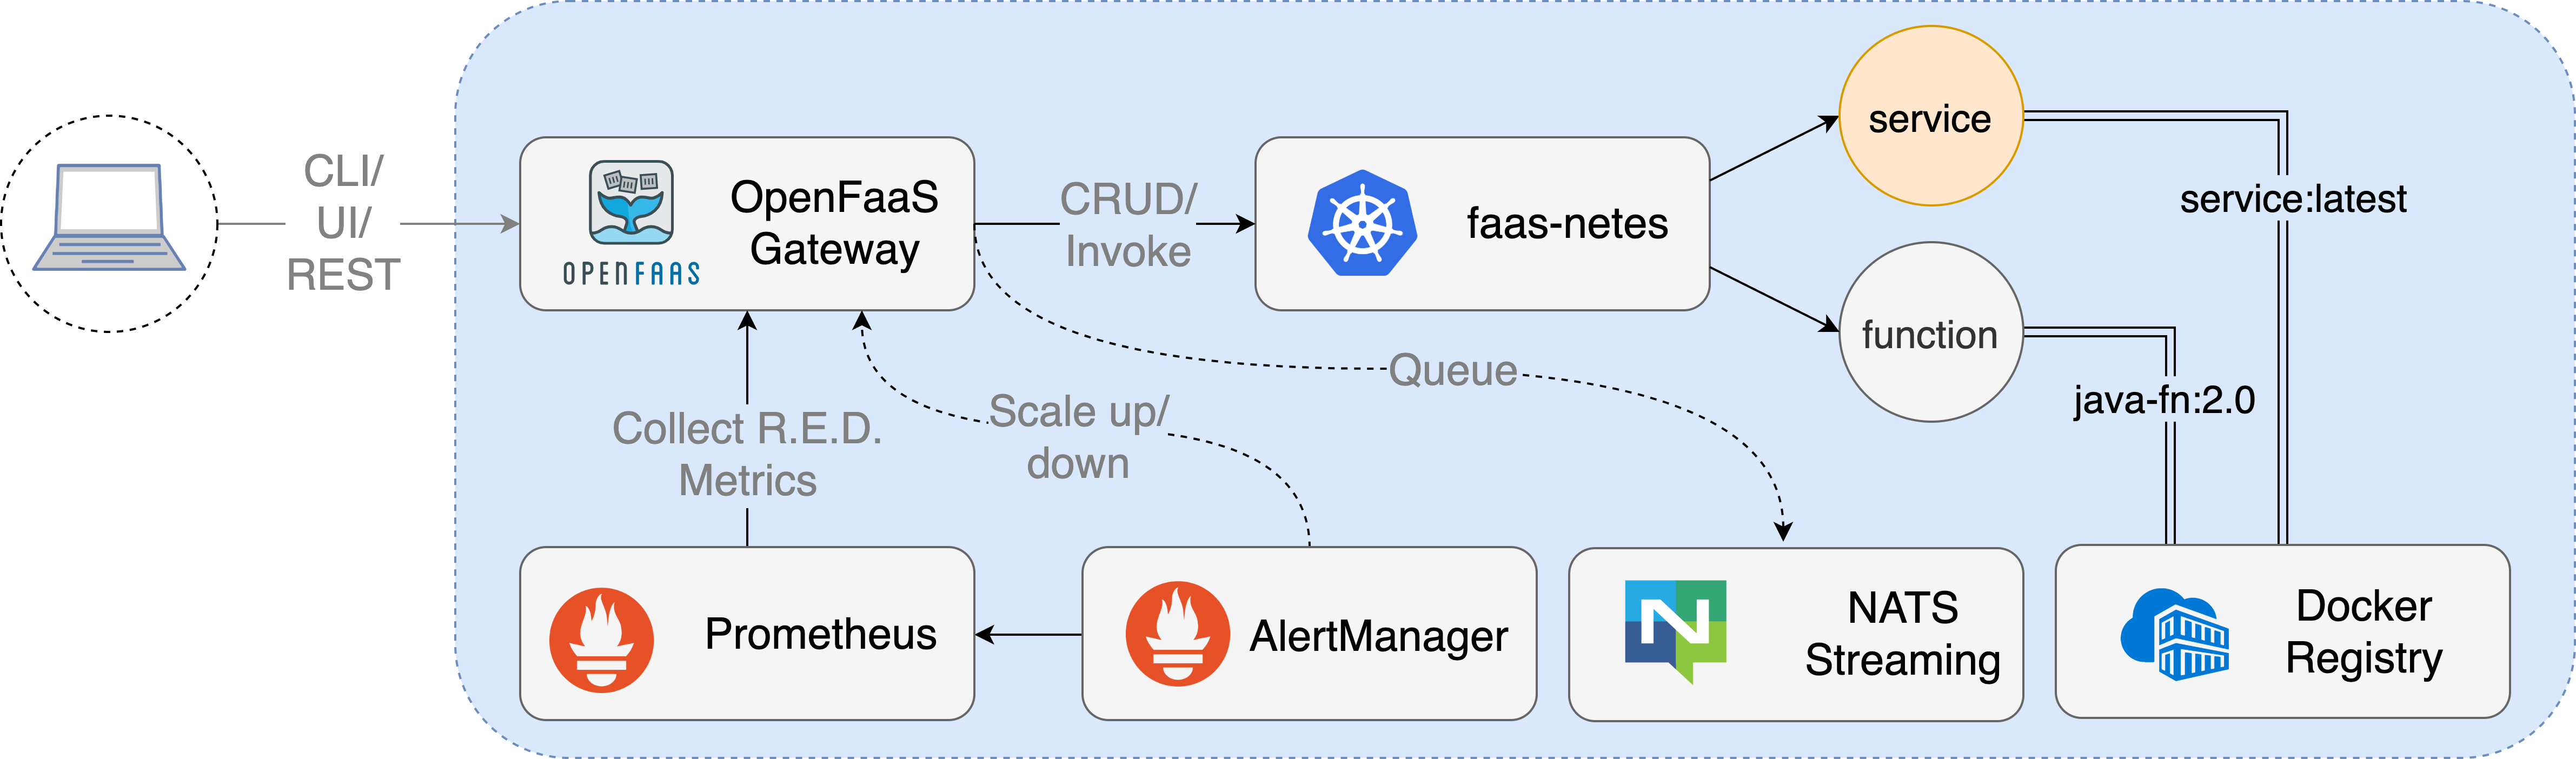
\includegraphics[width=\linewidth]{images/openfaas-workflow.png}
    \caption{OpenFAAS运行流程}
    \label{openfaas_workflow}
\end{figure}

它的架构如\cref{openfaas_arch}所示\cite{openfaas_arch},主要包含:

\begin{itemize}
    \item CI/GitOps层: 通过CI将用户编写的代码并部署到集群中
    \item 应用层: 包含网关、NATS和Prometheus,
    其中网关暴露REST形式的管理功能,NATS用于异步执行,Prometheus管理监控数据
    \item 基础层: 基于Kubernetes的运行时
\end{itemize}

\begin{figure}[ht!]
    \centering
    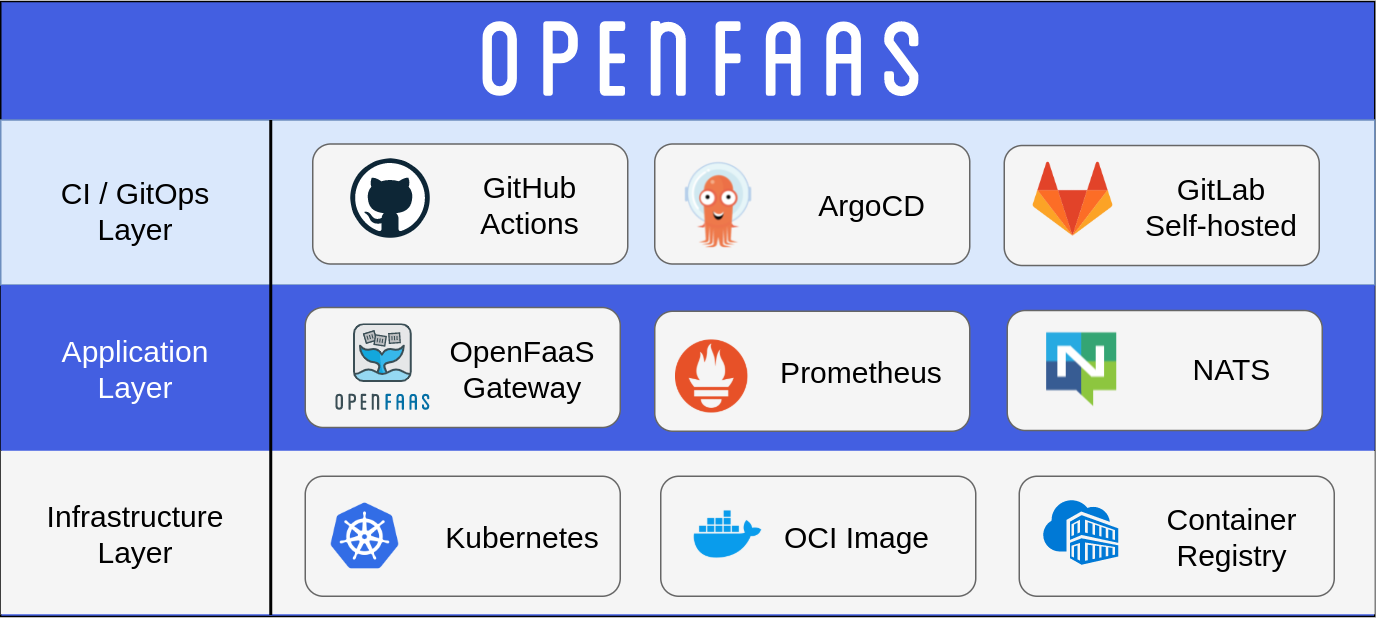
\includegraphics[width=\linewidth]{images/openfaas-overview.png}
    \caption{OpenFAAS架构概览}
    \label{openfaas_arch}
\end{figure}

\subsubsection{Knative}

\href{https://knative.dev/}{Knative}是由谷歌开源的一款serverless框架,
是CNCF的孵化项目。
Knative是基于Kubernetes的CRD(Kubernetes Custom Resource Definitions)和Istio实现的纯原生的架构,
包含以下的CRD:

\begin{itemize}
    \item Service: 负责管理整个计算负载的生命周期,控制其他资源的创建
    \item Route: 将网络映射到revision
    \item Configuration: 负责管理配置信息,更新配置时,会创建新的revision
    \item Revision: 计算负载的一个特定的版本实例(包含配置和代码等),能够根据负载自动进行伸缩
\end{itemize}

整个架构如\cref{knative_model}所示\cite{knative_concepts}。

\begin{figure}[ht!]
    \centering
    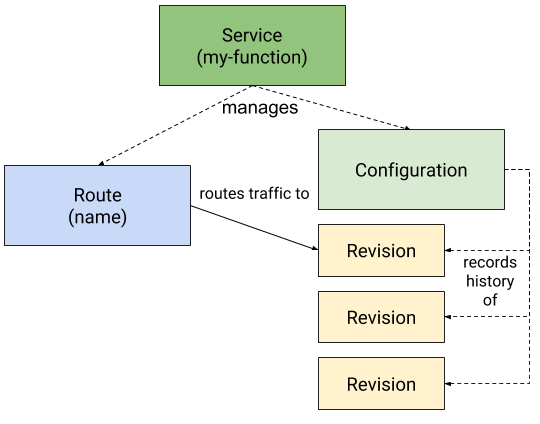
\includegraphics[width=\linewidth]{images/knative_object_model.png}
    \caption{Knative的模型}
    \label{knative_model}
\end{figure}

\subsubsection{Nuclio}
\href{https://nuclio.io/}{Nuclio}是一个开源的用户科学计算的serverless框架,
号称最快的serverless框架\footnote{"Real-time performance running up to 400,000 function invocations per second".},
并支持GPU加速。Nuclio开发的初衷是现有的serverless框架
不满足以下几点\cite{why_nuclio}:

\begin{itemize}
    \item 最小化CPU/GPU以及I/O使用、最大化并行度
    \item 原生能够支持多种数据源、触发方式、处理模型以及ML框架
    \item 有状态的函数处理(包含路径加速)
\end{itemize}

\begin{figure}[ht!]
    \centering
    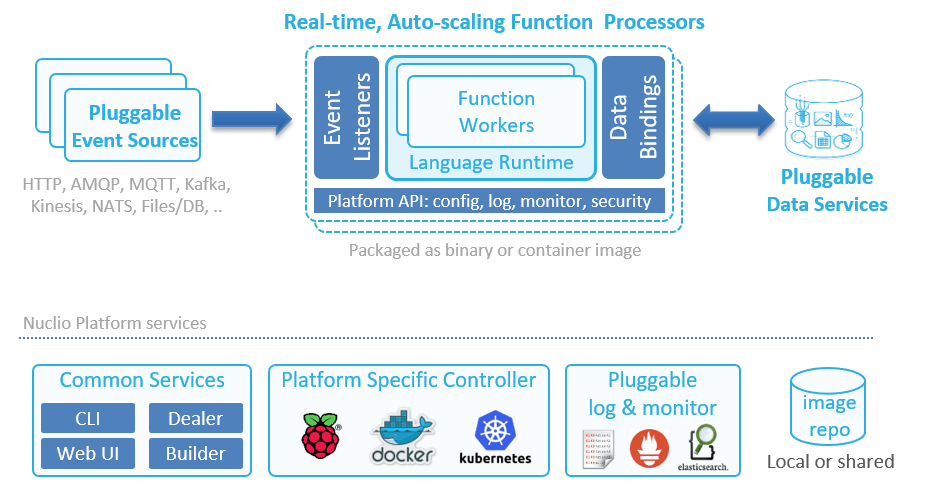
\includegraphics[width=\linewidth]{images/nuclio-arch.png}
    \caption{Nuclio的整体架构}
    \label{nuclio_model}
\end{figure}
